\section{Diagramma dei componenti}
Definiti gli aspetti visivi dell'applicazione si può procedere con una fase di design più avanzata,
che sfrutta profondamente i mockup stessi. \\
Il design architetturale dell'applicazione può essere rappresentato come l'unione di più blocchi, 
anche detti componenti, che messi insieme costruiscono le schermate dell'applicazione stessa. 
Ogni componente contiene al suo interno sia la parte logica che grafica necessaria al suo funzionamento. \\
Il diagramma dei componenti offre la possibilità di definire a priori gli oggetti che saranno centrali
nelle fasi di sviluppo, oltre a consentire una più semplice organizzazione del lavoro tra i membri
del gruppo. \\
Per semplicità di presentazione ogni schermata principale dell'applicazione è stata scomposta
nei suoi componenti principali, che sono stati poi rappresentati nel diagramma seguente. \\
In Figura \ref{fig:cd_home} è possibile osservare il diagramma dei componenti della schermata principale.
Degni di nota i componenti composti che racchiudono al loro interno altri componenti più piccoli. Questo 
perché alcuni componenti sono solo la composizione di alcuni più piccoli ma non per questo perdono la 
loro validità come tali. \\
Alcuni dei componenti riportano anche degli attributi; questo perché non tutti hanno un comportamento
indipendente da altri componenti, dunque è utile specificare quali dati essi devono
ricevere per poter funzionare correttamente. Non è detto che corrisponderanno fedelmente all'effettiva 
implementazione ma dovrebbero essere usati come linee guida. \\
È già possibile notare come i componenti di questa pagina corrispondano fedelmente a quelli del mockup. \\

\begin{figure}[h!]
    \centering
    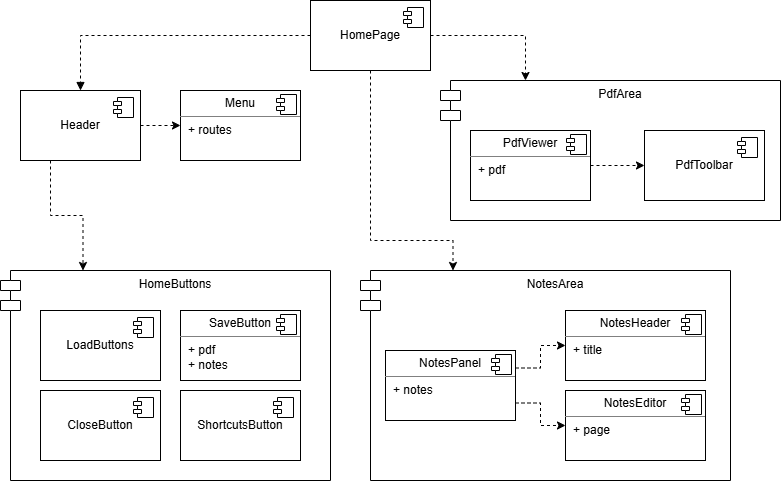
\includegraphics[width=1\textwidth]{diagrams/HomePage-CD.png}
    \caption{Diagramma dei componenti della pagina Home}
    \label{fig:cd_home}
\end{figure}

A seguire in Figura \ref{fig:cd_notes} e \ref{fig:cd_classes}
sono rappresentati i diagrammi dei componenti delle altre pagine principali dell'applicazione. \\
Qui invece è interessante come già alcuni componenti, seppure in forma differente, si ripetano in più pagine.
Questo è proprio il concetto di riusabilità dei componenti, che permette di velocizzare lo sviluppo
e mantenere una coerenza grafica tra le varie schermate. \\

\begin{figure}[h!]
    \centering
    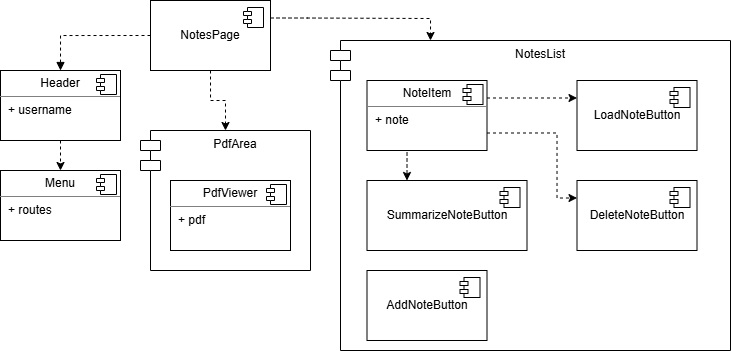
\includegraphics[width=1\textwidth]{diagrams/NotesPage-CD.png}
    \caption{Diagramma dei componenti della pagina delle note}
    \label{fig:cd_notes}
\end{figure}

\begin{figure}[h!]
    \centering
    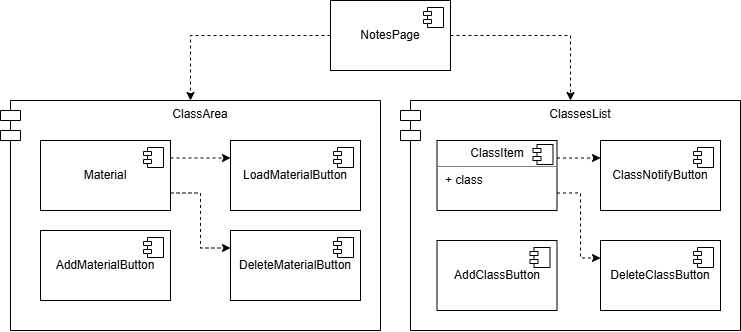
\includegraphics[width=1\textwidth]{diagrams/Classes-CD.png}
    \caption{Diagramma dei componenti della pagina delle classi}
    \label{fig:cd_classes}
\end{figure}

Proseguendo, in Figura \ref{fig:cd_profile} e \ref{fig:cd_login} sono rappresentati i diagrammi dei componenti
delle pagine del profilo e di login. \\
Questi diagrammi sono quelli più semplici in quanto le pagine stesse sono meno complesse
e contengono meno componenti. \\

\begin{figure}[h!]
    \centering
    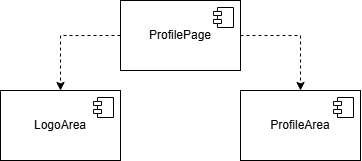
\includegraphics[width=1\textwidth]{diagrams/ProfilePage-CD.png}
    \caption{Diagramma dei componenti della pagina del profilo}
    \label{fig:cd_profile}
\end{figure}

\begin{figure}[h!]
    \centering
    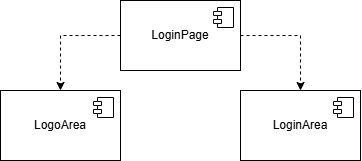
\includegraphics[width=1\textwidth]{diagrams/LoginPage-CD.png}
    \caption{Diagramma dei componenti della pagina di login}
    \label{fig:cd_login}
\end{figure}

Per concludere, sebbene i diagrammi abbiano una struttura gerarchica dovrebbero essere pensati come
macro-componenti a sé, nei quali è possibile anche una comunicazione bidirezionale. Le frecce
sono solo usate per indicare la direzione delle dipendenze funzionali tra i vari componenti.